\documentclass[titlepage,a4paper]{ctexart}
\usepackage{moreverb}
\usepackage{xcolor}
\usepackage{listings}
\definecolor{mygray}{gray}{0.85}
\setcounter{tocdepth}{2}
\lstset{numbers=left, firstnumber=0, basicstyle=\ttfamily\small, tabsize=8, keywordstyle=\color{blue!70}, commentstyle=\color{red!50!green!50!blue!50}, backgroundcolor=\color{mygray}, rulesepcolor=\color{red!20!green!20!blue!20},escapeinside=``, xleftmargin=2em,xrightmargin=2em, aboveskip=1em}
\usepackage[bookmarksdepth=3,bookmarksnumbered]{hyperref}

\ifx\shipout\UnDeFiNeD 
\else
\hypersetup{colorlinks=true,linkcolor=black,citecolor=black}
%\setCJKmainfont[BoldFont=SimHei]{SimSun}
%\setCJKmonofont{SimSun}
\fi 

\usepackage[top=2in, bottom=2in, left=1.4in, right=1.4in]{geometry}
\usepackage{graphicx}
\usepackage{subfigure}
\makeindex

\graphicspath{{figure/}{avatar/}}

\begin{document}
\newcommand{\HRule}{\rule{\linewidth}{0.5mm}}
\title{Smart Car Simulator (SCS) \\ Manual \& Programming Interface \\ 智能车仿真平台 \\ 使用手册及编程接口}
\author{swift studio \\ 思维伏特工作室}
\date{2013年4月}

\begin{titlepage}

\begin{center}
% Upper part of the page
\textrm{\LARGE Smart Car Simulator (SCS)}\\[0.5cm]
\textrm{\LARGE Manual \& Programming Interface}\\[0.8cm]
\textrm{\LARGE 智能车仿真平台 }\\[0.5cm]
\textrm{\LARGE 使用手册及编程接口}\\[0.5cm]
% Title
%\HRule \\[0.4cm]
%\huge \bfseries Lager brewing techniques}\\[0.4cm]
%\HRule \\[1.5cm]
\textrm{}\\[1.5cm]
\begin{tabular}{rr}
\textrm{API Version:} & \textrm{1.0} \\
\textrm{Library Version:} & \textrm{1.0.1} \\
\textrm{Document Version:} & \textrm{1.0.1} \\
\textrm{Track File Protocol Version:} & \textrm{0.9} \\
\end{tabular}

\vfill
% Bottom of the page
{\large
\textrm{swift studio \\ 思维伏特工作室} \\
2013年9月 \\[4.0cm]
}

\end{center}
\end{titlepage}

\tableofcontents
\newpage

\section{背景介绍}
SCS智能车仿真平台,以全国大学生智能车竞赛为背景,依照智能车竞赛规则建立仿真模型,旨在为广大参与智能车竞赛的参赛选手提供一个仿真智能车机械,验证软件控制算法的平台。

该平台以刚体模型库OpenDE和图形库OpenGL为基础,描述并绘制智能车以及赛道的机械模型,仿真智能车行进的物理过程。

该平台自2012年8月开始开发以来,备受同学老师以及广大车友的关怀。直到2013年8月1日正式版发布,这一年以来,在广大车友的共同帮助下,SCS的许多不足得到了改进,许多bug得到了修复。在SCS日趋稳定的形势下,我们迎来了SCS-1.0.1的发布。

本次发布的SCS-1.0.1版在上一个版本基础上修复了一些bug,调节了少数细节,基本没有太大变化。严格按照第八届智能车竞赛规则,并结合第八届智能车竞赛举办过程的实际情况,提供对智能车竞赛三个组别的车模、传感器、赛道的仿真。

\section{目标用户}
本软件面向参与智能车竞赛的参赛选手,以及所有对车辆机械模型、运动学模型、路径规划算法感兴趣的老师、同学以及相关研究人员。

本文档面向对本软件感兴趣的用户,向其介绍本软件的开发背景、发展状况。本文档面向希望学习本软件的用户,向其介绍本软件的设计思路、整体架构。本文档面向所有使用本软件的用户,向其提供接口说明。

本文档的背景介绍部分假设用户了解智能车竞赛。本文档的系统架构部分假设用户具有软件开发经验,熟悉软件开发一般流程和软件的一般架构,大致了解程序、库等基本概念。本文档的界面操作、终端信息两部分假设用户具有日常使用计算机的基本技能,并对终端操作具有简单的了解。本文档的接口函数部分假设用户具有C语言编程经验,熟悉C语言调用库函数的方法。本文档的新建工程部分假设用户熟悉函数库的调用方法,了解向编译器或开发环境添加依赖关系的方法。本文档的编辑赛道部分假设用户具有基本的文件编写能力。本文档的样例函数部分假设用户具有C语言程序的阅读能力,以及查阅OpenGL文档的能力。


\section{最低配置}
\begin{center}
\begin{tabular}{lll}
\hline
项目	& & 参数 \\
\hline
CPU主频	& & 1GHz \\
内存	& & 128M \\
显存	& & 128M \\
OpenGL	& & 2.1  \\
键盘	& & 必要 \\
鼠标	& & 不必要 \\
\hline
\end{tabular}
\end{center}

\section{系统架构}
\subsection{发布形式}
本软件以源代码的形式发布。发布包中包含本软件的所有源代码,以及Linux、VS2008、VS2010环境下的工程文件。本软件编译后生成静态链接库,由用户编写主程序以及控制算法,并调用库所提供的函数接口的形式来实现仿真。

\subsection{逻辑结构}
平台以OpenDE为物理模型底层,向OpenDE描述智能车的机械结构以及赛道的形状信息,并从OpenDE读取物理模型的各项参数。以OpenGL为图形底层,根据从OpenDE中返回的物理信息渲染图像并显示到窗口中。其中窗口管理由可跨平台的freeglut实现。
用户可调用平台提供的接口,读取仿真传感器的值,并据此编写决策算法,调用仿真的电机舵机的接口函数,输出控制信号以控制小车。
\begin{figure}[!htbp]
\centering
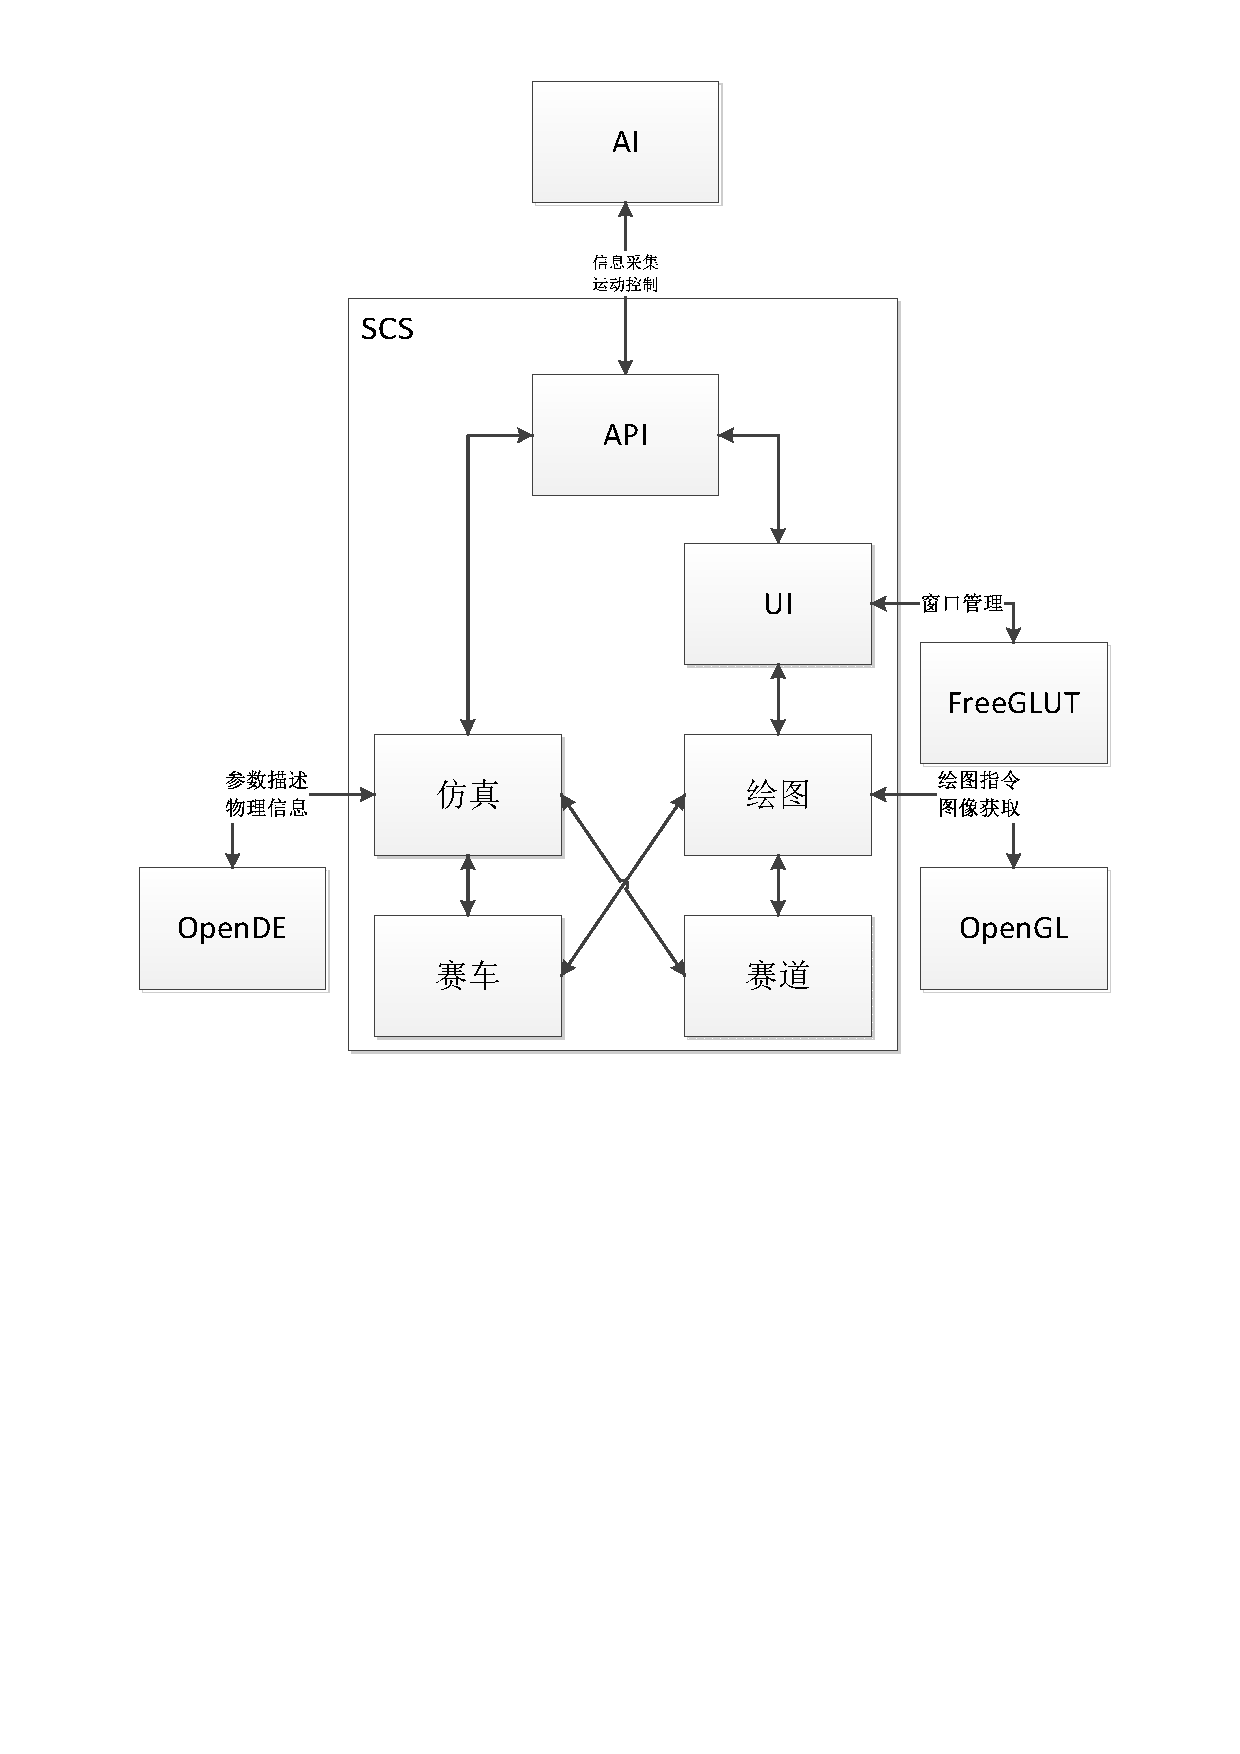
\includegraphics[width=0.65\textwidth]{logic.pdf}
\caption{逻辑结构图}
\end{figure}
%<image src="logic.png" name = "逻辑结构图"><居中>

\subsection{时序结构}
平台在初始化时获取用户决策算法的函数指针,作为回调函数,此后进入主循环。在主循环中,首先对物理过程进行仿真;然后根据仿真的结果绘制并显示图像;再根据物理参数计算传感器的测量值;最后调用用户回调函数。如此完成一轮主循环。该循环周而复始,直到使用者退出。
对于用户决策算法,其典型结构分为三步:首先调用接口读取传感器值;而后根据传感器信息计算控制信息;最后调用接口输出控制量。此部分结构相当于单片机中的定时中断,或场中断。由用户自行编写。
\begin{figure}[!htbp]
\centering
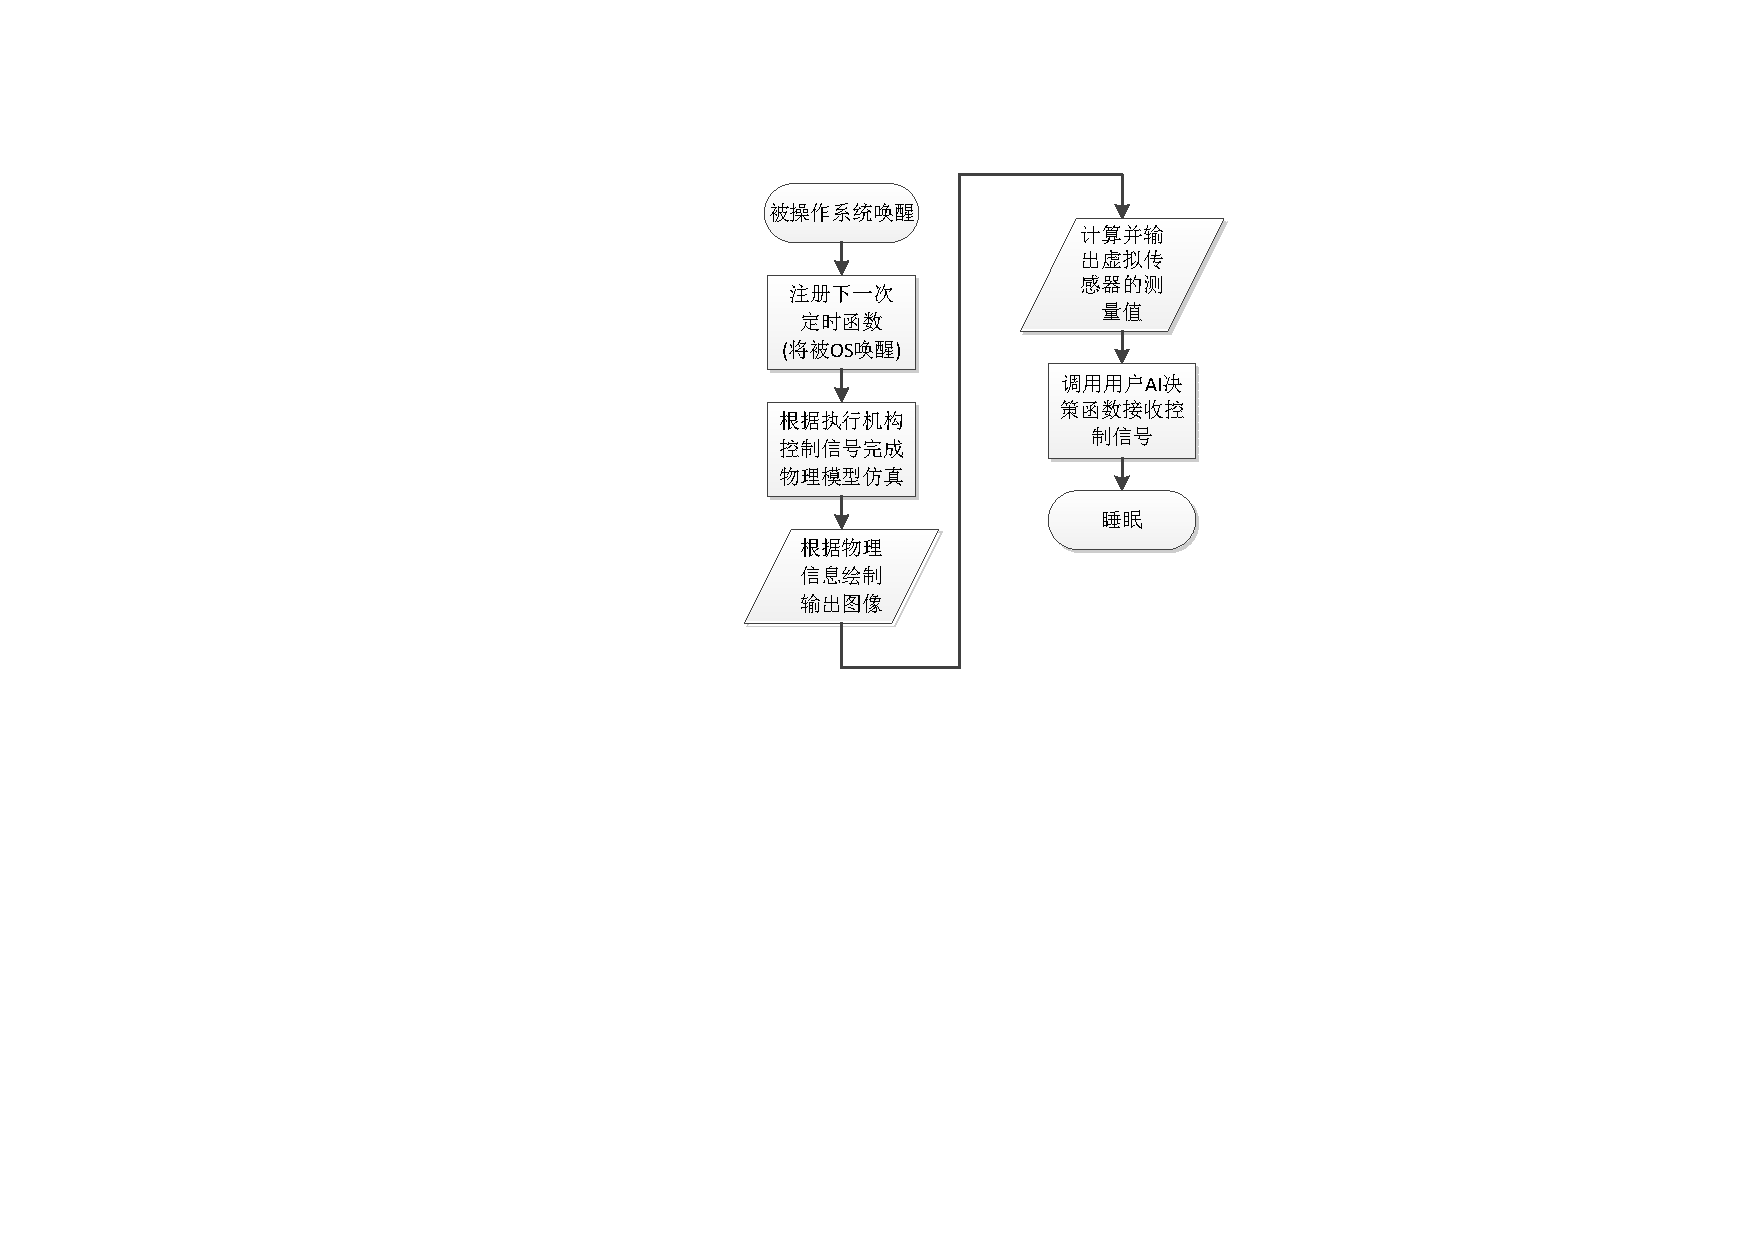
\includegraphics[width=0.60\textwidth,angle=270]{time.pdf}
\caption{时序结构图}
\end{figure}
%<image src="time.png" name = "时序结构图"><居中>

\subsection{数据结构}
在所有传递物理标量的接口函数中,舵机电机控制函数的参数为整形。其余全为双精度浮点型。若所传递的物理量为矢量,但仅其某一分量有意义,也当做标量传递。
对于需要传递矢量的接口函数,其矢量被声明为sVector类。声明如下:

\begin{lstlisting}[language=C++]
class sVector {
private:
        double x;
        double y;
        double z;
        double len;
public:
        sVector ();
        sVector (double x, double y, double z);
        double GetX ();
        double GetY ();
        double GetZ ();
        void SetX (double x);
        void SetY (double y);
        void SetZ (double z);
        void set (double x, double y, double z);
        double CalcLen ();
        double GetLen ();
        sVector Normalize ();
        sVector operator+(sVector v);
        sVector operator-(sVector v);
        sVector operator*(double n);
        friend sVector operator * (double n, sVector v);
        sVector operator / (double div);
        sVector operator += (sVector v);
        sVector operator -= (sVector v);
        sVector operator *= (double n);
        sVector operator /= (double n);
        sVector RotateZ (double theta);
        bool operator == (sVector v);
        bool operator != (sVector v);
        void print();
};
\end{lstlisting}
%(上面将会粘贴一段新的代码,文本内部自带tab缩进)

此类不仅可以在参数传递时使用,也可以在决策算法中供用户使用。

此矢量类取车身为自然坐标系,取国际标准基本单位及其导出单位为单位。
\begin{figure}[!htbp]
\hypertarget{coord}{}%
\centering
\subfigure[]{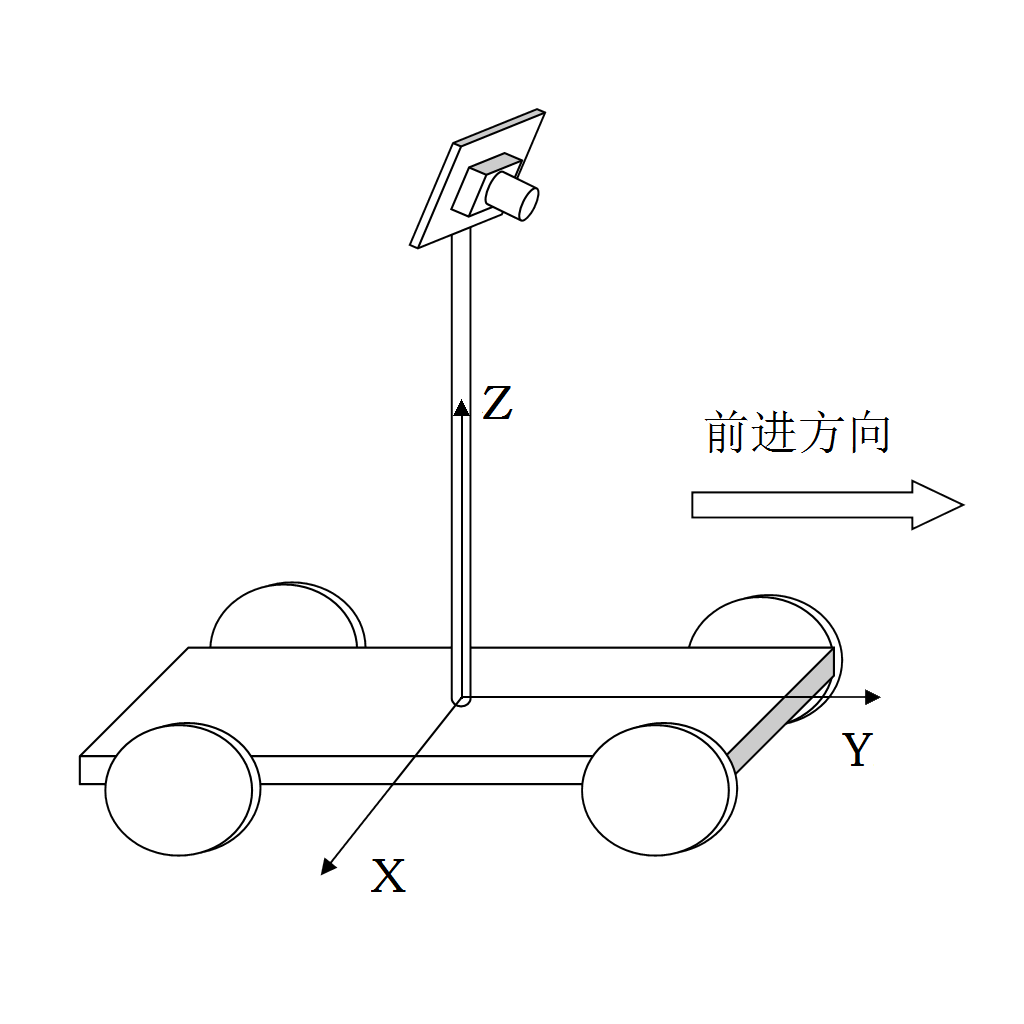
\includegraphics[width=0.45\textwidth]{coordinate.png}}
\subfigure[]{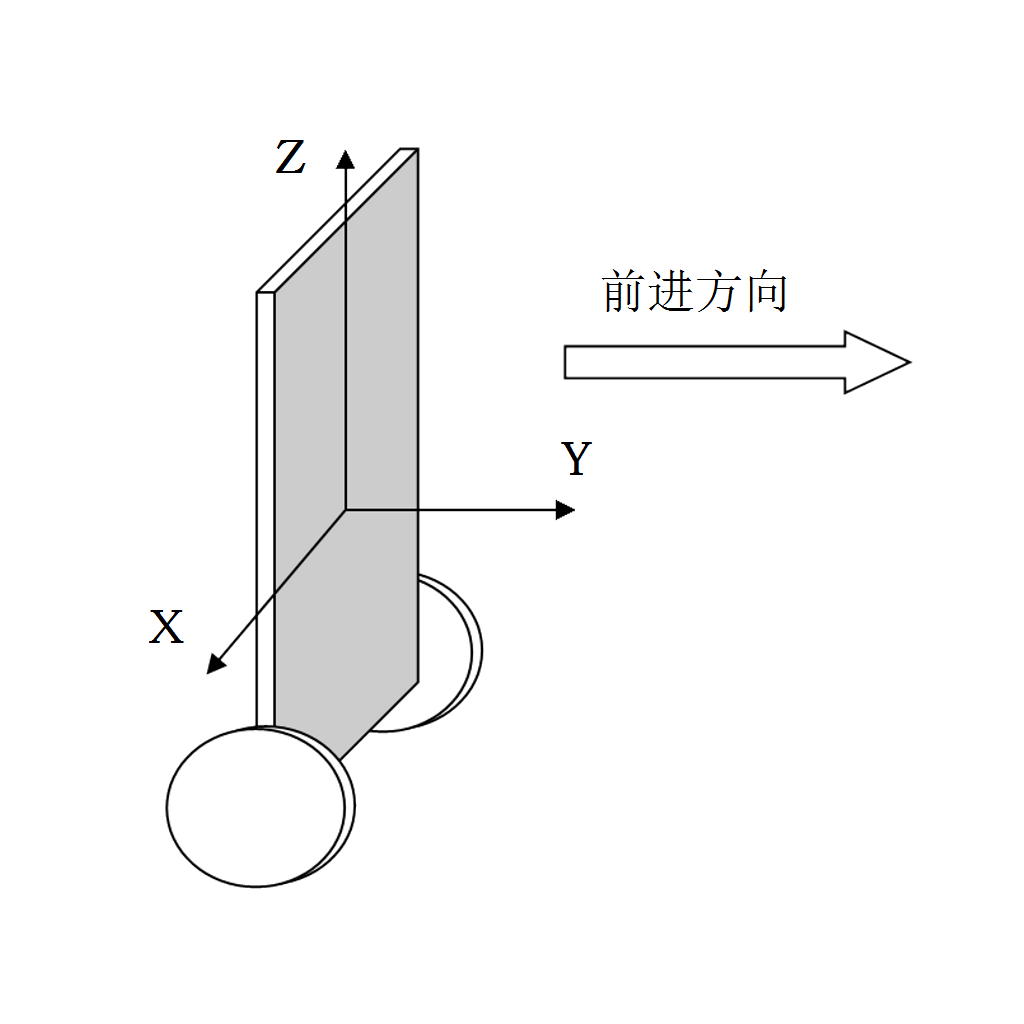
\includegraphics[width=0.45\textwidth]{coordinate_balance.png}}
\caption{自然坐标系}
\end{figure}
%<image src="coordinate.png" name = "自然坐标系(a)"><靠左>
%<image src="coordinate_balance.png" name = "自然坐标系(b)"><靠右>
%<上述两图在同一行>

以下枚举类型表示小车的型号
\begin{lstlisting}[language=C++]
enum CarType {
	camera,electromagnetic,balance,
};
\end{lstlisting}
\newpage
\section{界面操作}
\subsection{界面布局}
下图为SCS平台主界面。小车在视场中央,下面是赛道。地面有一米见方的网格线。在屏幕下方的蓝色条表示小车舵机当前转角。屏幕右侧蓝、绿、红色带分别表示当前电机功率、轮子转速、小车质心速度,对于绿、红色带,旁边红色的标尺每一格表示1m/s。
\begin{figure}[!htbp]
\centering
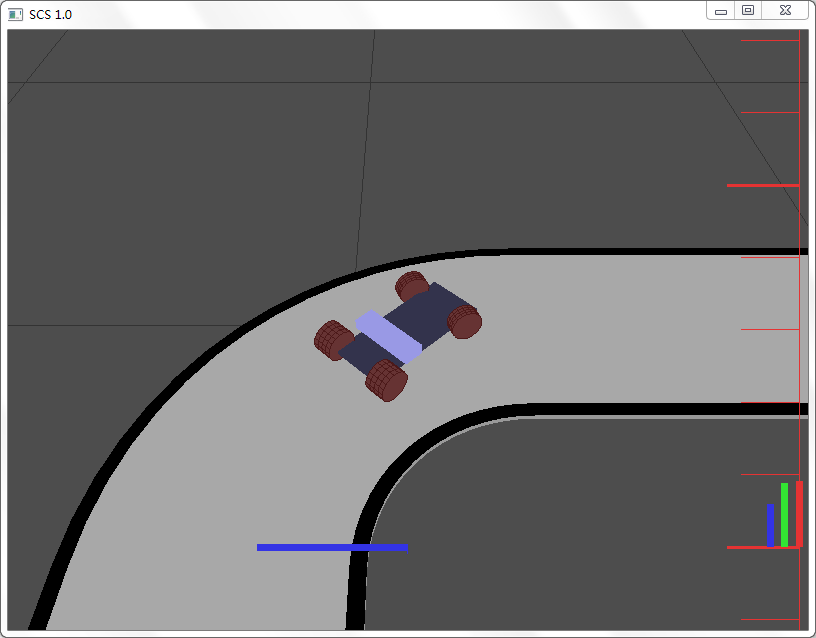
\includegraphics[width=0.75\textwidth]{window.png}
\caption{窗口界面布局}
\end{figure}
%<image src="window.png" name="窗口界面布局"><middle>
\subsection{运行模式}
仿真平台共有三种运行模式:AI模式,手动驾驶模式,调试模式。

AI模式即由决策回调函数控制小车寻路的模式。只要在进入scsMainLoop()前注册决策回调函数即进入该模式。

手动驾驶模式由使用者通过键盘控制小车的行驶。在主界面(非控制台界面)按“A”键即进入手动驾驶模式。如果在进入scsMainLoop()前没有注册决策回调函数,则直接进入手动驾驶模式。

调试模式下决策算法继续运行,但此时其对舵机与电机的操作无效,转而由键盘控制。在主界面按“D”键即可进入调试模式。

\subsection{鼠标操作}
可拖动鼠标左键调节水平视角,拖动右键调节视点高度,拖动中键调节视点位置,滑动中键推拉远近。

\subsection{键盘操作}
各个按键及其对应的操作见下表
\begin{center}
\begin{tabular}{ll}
\hline
按键	& 操作 \\
\hline
F1	& 输出帮助信息 \\
$\sim$  & 俯视视角 \\
1	& 第一人称视角 \\
2	& 鸟瞰视角 \\
3	& 跟随鸟瞰视角 \\
4	& 跟随视角 \\
5	& 后跟随视角 \\
6	& 跟随俯视视角 \\
7       & 软跟随视角 \\
0       & 自由视角 \\
A	& 开启或关闭手动驾驶模式 \\
D       & 开启或关闭调试模式 \\
R	& 将小车移回初始位置 \\
T       & 将小车移回初始位置,并沿反方向跑 \\
C	& 清除尾迹 \\
+	& 加速仿真 \\
$-$	& 慢速仿真 \\
O	& 恢复正常仿真速度 \\
P       & 暂停仿真 \\
V	& 恢复原始视角(消除鼠标拖动对视角造成的改变) \\
方向键	& 在手动驾驶模式下控制小车 \\
ESC	& 退出 \\
\hline
\end{tabular}
\end{center}

上述按键均不区分大小写。
\newpage
\section{终端信息}
\subsection{正常信息}
控制台首先会输出初始化信息、版本信息,接着会输出创建虚拟环境的提示信息。在每次按下键盘按键时会输出所按的键以及所产生的效果。在小车每跑完一圈后会显示当前圈数和时间、平均速度等信息。小车在第一次冲线时会显示圈数为0,此时的时间以及平均速度表示从起点到第一次冲线的时间及平均速度。

\subsection{错误信息}
当程序运行出错时,会输出错误信息,其含义如下表:
\begin{center}
\begin{tabular}{ll}
\hline
错误信息 & 含义 \\
\hline
You have not register this software & 尚未注册本软件,请阅读license \\
There is no AI function	& 未注册决策算法回调函数 \\
There is no track file  & 尚未注册赛道文件 \\
There is no route	& 清除并不存在的尾迹 \\
Unknown command	& 未知的按键 \\
Can not open track file	& 无法打开赛道文件 \\
Unrecognized track type & 无法识别的赛道类型 \\
The Track is too long to draw	& 赛道太长以至于无法绘制 \\
Can not connect to be a circle	& 赛道无法连成回路 \\
The security of path is too high/low	& 最优路径安全系数过高/过低 \\
Normalize zero vector	& 对零向量进行归一化操作 \\
SetMotor: Too high/low!	& 电机输入电压过高/过低 \\
SetServoDir: Too high/low & 舵机角度过大/过小 \\
\hline
\end{tabular}
\end{center}

上述问题的解决办法详见后文。
\newpage
\section{接口函数}

\subsection{初始化}
\subsubsection{sSetCar}
\begin{lstlisting}[numbers=none]
void sSetCar (CarType cartype);
\end{lstlisting}
\par \emph{cartype 小车的型号}

设置所要仿真的车的型号,默认仿真摄像头车 \\

\subsubsection{sSetAiFunc}
\begin{lstlisting}[numbers=none]
void sSetAiFunc (void f());
\end{lstlisting}
\par \emph{f    决策算法函数指针}

注册决策算法回调函数。该函数将每隔20ms调用一次。若未注册,则平台只能运行在手动模式下。 \\

\subsubsection{sSetInitFunc}
\begin{lstlisting}[numbers=none]
void sSetInitFunc (void f());
\end{lstlisting}
\par \emph{f    初始化函数指针}

注册初始化回调函数。该函数在程序运行一开始时被调用一次,在每次小车回复初始位置时被调用一次。 \\

\subsubsection{sSetTrack}
\begin{lstlisting}[numbers=none]
sSetTrack (const char * s);
\end{lstlisting}
\par \emph{s    赛道文件名字符串首地址}

设置赛道文件,s所指向的字符串即为赛道文件路径。可用相对路径,也可用绝对路径。不调用此函数不能运行仿真平台。 \\

\subsubsection{scsMainLoop}
\begin{lstlisting}[numbers=none]
void scsMainLoop (int * argc, char *argv[]);
\end{lstlisting}
\par \emph{argc  指向主函数的argc参数的指针}
\par \emph{argv  同主程序argv参数}

进入SCS主循环,需将main函数的参数传入,注意argc是指针。进入此函数后不可跳出,只可结束程序。此函数后面的代码不会被执行。 \\

\subsection{功能开关}
\subsubsection{sEnableRoute}
\begin{lstlisting}[numbers=none]
void sEnableRoute ();
\end{lstlisting}

开启尾迹功能。此功能可将小车经过的路线画出来。 \\

\subsubsection{sEnableReverse}
\begin{lstlisting}[numbers=none]
void sEnableReverse ();
\end{lstlisting}

开启反跑功能。小车将沿着相反的方向跑,即摄像头组正跑,电磁组反跑。 \\

\subsubsection{sEnableMiddleLine}
\begin{lstlisting}[numbers=none]
void sEnableMiddleLine ();
\end{lstlisting}

显示赛道中心线。若小车型号为电磁车,则默认开启此功能,否则默认关闭。 \\

\subsection{物理参数}
\subsubsection{sSetCamera}
\begin{lstlisting}[numbers=none]
void sSetCamera (sVector pos);
\end{lstlisting}
\par \emph{pos   摄像头坐标}

设置摄像头相对于小车\hyperlink{coord}{自然坐标系}的位置。默认值是 sVector (0.0, 0.0, 0.3),即小车几何中心正上方30厘米处。 \\

\subsubsection{sSetCCD}
\begin{lstlisting}[numbers=none]
void sSetCCD (sVector pos);
\end{lstlisting}
\par \emph{pos   线性CCD坐标}

设置线性CCD相对于小车\hyperlink{coord}{自然坐标系}的位置。默认值是 sVector (0.0, 0.0, 0.3),即小车几何中心正上方30厘米处。 \\

\subsubsection{sSetDepressionAngle}
\begin{lstlisting}[numbers=none]
void sSetDepressionAngle (double depressionangle);
\end{lstlisting}
\par \emph{depressionangle 俯角}

设置摄像头以及线性CCD的俯角,默认的俯角是30°。 \\

\subsubsection{sSetBatteryPosition}
\begin{lstlisting}[numbers=none]
void sSetBatteryPosition (sVector pos);
\end{lstlisting}
\par \emph{pos   电池位置}

设置电池相对于小车\hyperlink{coord}{自然坐标系}的位置。对于摄像头车,默认值为sVector (0.0, 0.05, 0.02),对于电磁车,默认值为sVector (0.0, -0.05, 0.02),对于光电平衡车,默认值为sVector (0.0, -0.01, -0.03)。 \\

\subsection{运动控制}
\subsubsection{sSetMotor}
\begin{lstlisting}[numbers=none]
void sSetMotor (int voltage);
void sSetMotorL (int voltage);
void sSetMotorR (int voltage);
\end{lstlisting}
\par \emph{voltage 电压}

控制电机旋转,sSetMotor()使得左右电机得到相同的参数,后二者可分别控制两电机。参数可正可负,单位为与伏特正相关的某个量。 \\

\subsubsection{sSetServoDir}
\begin{lstlisting}[numbers=none]
void sSetServoDir (int dir);
\end{lstlisting}
\par \emph{dir   舵机偏转角度}

控制舵机偏转角度,dir表示角度,范围为正负一百之间,单位为与角度成正比的某个量。 \\

\subsection{传感器}
\subsubsection{sGetSpeed}
\begin{lstlisting}[numbers=none]
double sGetASpeedL ();
double sGetASpeedR ();
double sGetASpeed ();
double sGetSpeedL ();
double sGetSpeedR ();
double sGetSpeed ();
\end{lstlisting}

读取后轮转速,带A的表示读取的是弧度制单位,否则是角度值单位。结尾是L表示读取的是左轮转速,结尾是R表示读取的是右轮转速。既不是L也不是R表示读取的是两轮平均转速。 \\

\subsubsection{sGetAngularSpeed}
\begin{lstlisting}[numbers=none]
sVector sGetAngularSpeed ();
\end{lstlisting}

读取角速度,返回为一向量,表示其角速度矢量。 \\

\subsubsection{sGetAcc}
\begin{lstlisting}[numbers=none]
sVector sGetAcc ();
\end{lstlisting}

读取小车几何中心的加速度,且在其竖直分量上加上向上的重力加速度$9.8 \mathrm{m/s^2}$再返回。 \\

\subsubsection{sGetMagnetic}
\begin{lstlisting}[numbers=none]
sVector sGetMagnetic (sVector pos);
\end{lstlisting}
\par \emph{pos   电磁传感器位置}

返回相对于小车底盘几何中心pos位置处的磁感应强度。假设赛道中心线通以稳恒电流,且该传感器直接传感磁感应强度。注意:实际赛道是通以交变电流,传感器是测的磁通量的变化率。此处用更简单的模型代替,其测量值与实际传感器所得信号成正比。单位取与特斯拉成正比的某个量。

电磁传感器的位置需要每次传感时都输入。与摄像头和线性CCD比较,后二者只要在使用前设定好初始位置即可。

被测的位置会在主界面上用小球表示,每个控制周期最多只能调用本函数128次,超过128次调用则只能返回零向量。 \\


\subsubsection{sGetReedSwitch}
\begin{lstlisting}[numbers=none]
int sGetReedSwitch ();
\end{lstlisting}

返回干簧管的状态,1表示干簧管在起止线附近,否则表示干簧管不在起止线附近。若车以5米每秒以上的速度冲过起止线,则有可能无法检测到。\\

\subsection{图像}
\subsubsection{sGetGraph}
\begin{lstlisting}[numbers=none]
void sGetGraph (unsigned char graph[GRAPH_HEIGHT][GRAPH_WIDTH]);
\end{lstlisting}
\par \emph{graph  二维图像数组首地址}

获取图像,将二维数组首地址传入,该函数将图像信息写入数组中。注意一定要保证二维数组的大小是GRAPH\_HEIGHT行,GRAPH\_WIDTH列。若小于该大小,将发生未知错误且不会给出任何提示。其中GRAPH\_HEIGHT和GRAPH\_WIDTH的值定义在头文件中,请勿改动。每个像素由8位无符号变量表示,0表示全黑,255表示全白。无色相及饱和度,仅有灰度。注意:在第一人称视角下可以看到,赛道外地面的背景颜色和赛道颜色是完全相同的,此函数返回的图像正是第一人称视角看到的图像经过分辨率调整后所得。在其他视角下赛道背景为深灰色,此函数返回的图像背景仍然为白色。返回图像的像素长宽比为4:3,与实际的图像的长宽比相符。虚拟摄像头视场的水平张角约80°,垂直张角为45°。 \\

\subsubsection{sGetLine}
\begin{lstlisting}[numbers=none]
void sGetLine (unsigned char line[GRAPH_WIDTH]);
\end{lstlisting}
\par \emph{line  一维图像数组首地址}

读取一行,使用方法同sGetGraph。本函数读取的数据相当于sGetGraph函数返回的图像的正中间的那一行,视场张角约80°。 \\

\subsection{客户窗口}
\subsubsection{sEnableCustomWindow}
\begin{lstlisting}[numbers=none]
void sEnableCustomWindow ();
void sEnableCustomWindow (int num);
\end{lstlisting}
\par \emph{num  客户窗口的个数}

开启num个客户窗口,编号为0到num-1,num最大不可超过16。用户可以使用OpenGL向对应的窗口绘制图像,可以使用GLUT控制这些窗口。num的缺省值为1。\\

\subsubsection{sSetDisplayFunc}
\hypertarget{h672}{}%
\begin{lstlisting}[numbers=none]
void sSetDisplayFunc (void f());
void sSetDisplayFunc (void f(), int num);
\end{lstlisting}
\par \emph{f   绘制回调函数}
\par \emph{num  上述回调函数所对应的客户窗口编号}

对编号为num的客户窗口注册绘制回调函数,num的缺省值为0,若num超过16,也会被置为0。该函数将在回调函数调用后立即被调用。调用过程如下:
\begin{lstlisting}[language=C++]
glutSetWindow (WinCustom);
glClear (GL_COLOR_BUFFER_BIT);
glLoadIdentity ();
glColor3d (1.0,1.0,1.0);

f ();

glFlush ();
glutSwapBuffers ();
\end{lstlisting}

\newpage
\section{新建工程}
由于不同的开发环境具体过程略有不同,在此只粗略地描述大体流程。

\subsection{配置依赖关系}
将include目录添加到头文件搜索目录中,将lib目录添加到库文件搜索目录中,将scs.lib ode\_double.lib freeglut\_static.lib库文件设置到依赖关系中。

\subsection{编写主函数}
新建C语言源文件,在文件中包含scs.h头文件,在主函数中调用初始化函数,最后调用主循环函数scsMainLoop()。

\subsection{编写决策函数}
调用传感器及运动控制的接口函数编写决策函数,并用sSetAiFunc()将其函数指针注册为回调函数。
\newpage
\section{编辑赛道}
\subsection{文件结构}
赛道文件为文本文件,扩展名为trk。赛道文件以若干个“段”(segment)表示赛道。每一段只能是直道或弯道二者之一。相邻两段相接处保证位置相同切线方向相同。赛道可以形成封闭回路,也可以不封闭。赛道可以是简单曲线,也可以是复杂曲线,例如自交。

若赛道共有n段,则赛道文件共n+2行。其中第一行是一个实数,表示起止线沿赛道中心线到坐标原点的距离,该值可正可负。接下来n行每行表示一个段。最后一行是两个数0,中间用空白字符隔开。

中间n行每行有2到4个元素。前两个元素是两个实数,表示赛道的长度和半径。第三个元素表示本段是否是特殊赛道,可以没有第三个元素。第四个元素是注释,以双斜杠开头,可以没有。相邻两个元素用空白字符隔开。
\subsection{直道}
如果第二个元素半径为0,则表示本段为直道,第一个元素表示直道的长度,单位是厘米。第一段赛道必须是一段2米以上的直道。
\subsection{弯道}
如果第二个元素半径大于赛道宽度的一半,则表示本段为弯道。半径的单位是厘米,若为正表示左拐,反之表示右拐。此时第一个元素表示弯道所扫过的角度,单位为度。
\subsection{特殊}
每行若无第三个元素,则表示本段为普通赛道。若为“\textasciicircum”(SHIFT+6),表示本段为坡道。此时赛道长度表示坡道在地面投影的长度。坡道长度最短为20cm,不足20cm以20厘米计算。第一个坡道为上坡,第二个为下坡,以此类推。若第三个元素为“.”(英文句号),则表示本段为虚线,虚线只能出现在弯道上但不仅限于小S弯,若出现在直道上将被忽略。若为一个字符“+”,表示本段为非平衡组的障碍,若为一个字符“*”,表示本段为平衡组的障碍。若仿真小车类型设置为平衡组,则“+”将被忽略;若仿真小车类型设置为非平衡组,则“*”将被忽略。障碍将高出普通赛道0.5厘米,非平衡组障碍边缘是45°斜面,平衡组障碍边缘是30°斜面。
\subsection{其他}
每行最后可以有双斜杠开头的注释。
每行不得超过255个字符。
可以有空白行,平台将忽略。
推荐用制表符作为相邻两元素间的间隔。
\subsection{样例赛道}
\subsubsection{样例一}
\begin{lstlisting}
50		// 起止线沿赛道中心线到原点的距离
100	0	// 直道
180	50	// 左拐
100	0	// 直道
180	50	// 左拐
0	0	// 结束
\end{lstlisting}
\begin{figure}[!htbp]
\centering
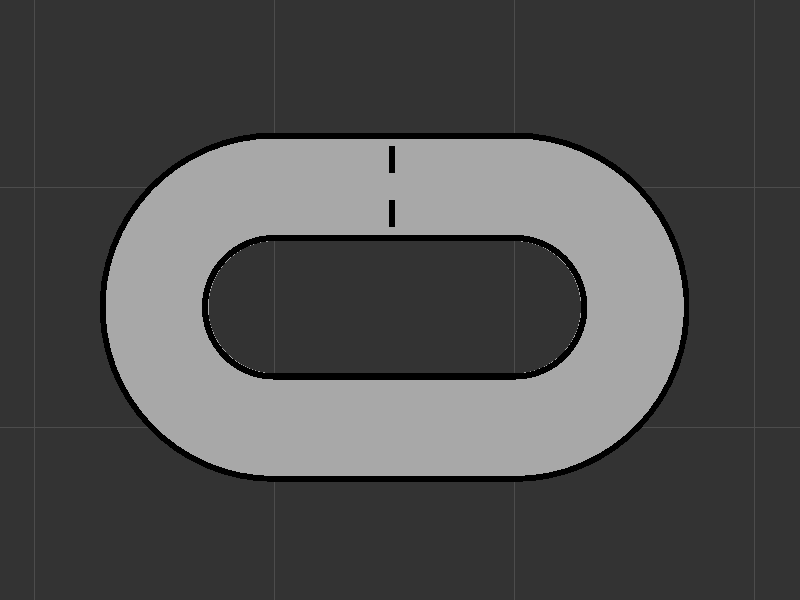
\includegraphics[width=0.80\textwidth]{demo1.png}
\caption{样例一}
\end{figure}
\newpage
%<image src="demo1" name = "样例一"><middle>
\subsubsection{样例二}
\begin{lstlisting}
50
100	0
10	0	+	// 障碍
10	0
10	0	+	// 障碍
10	0
10	0	+	// 障碍
100	0
180	50
100	0
50	0	^	// 上坡
100	0
50	0	^	// 下坡
100	0
180	50
149	0
0	0
\end{lstlisting}
\begin{figure}[!htbp]
\centering
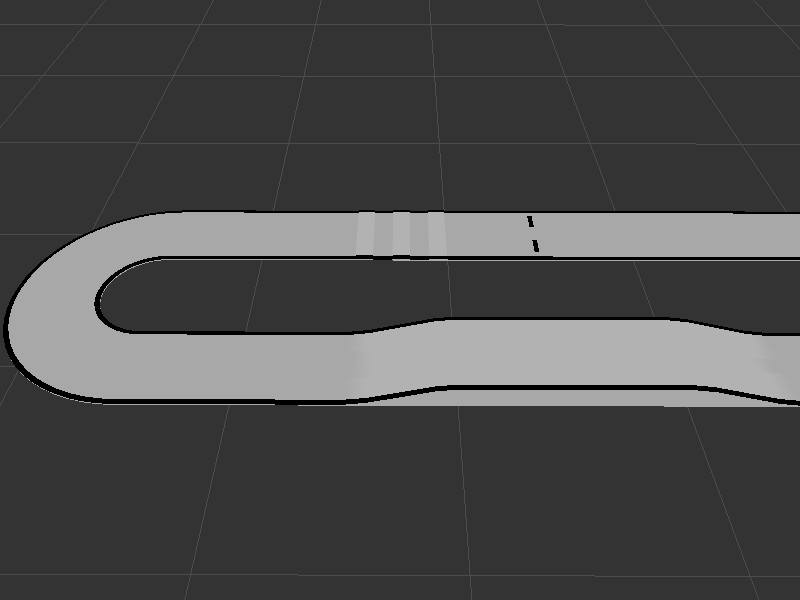
\includegraphics[width=0.80\textwidth]{demo2.png}
\caption{样例二}
\end{figure}
%<image src="demo2" name = "样例二"><middle>
\subsubsection{样例三}
\begin{lstlisting}
50
100	0
30	50	.	// 虚线
60	-50	.
60	50	.
60	-50	.
60	50	.
60	-50	.
30	50	.

180	-100
500	0
270	50
200	0
90	-50

0	0
\end{lstlisting}
\begin{figure}[!htbp]
\centering
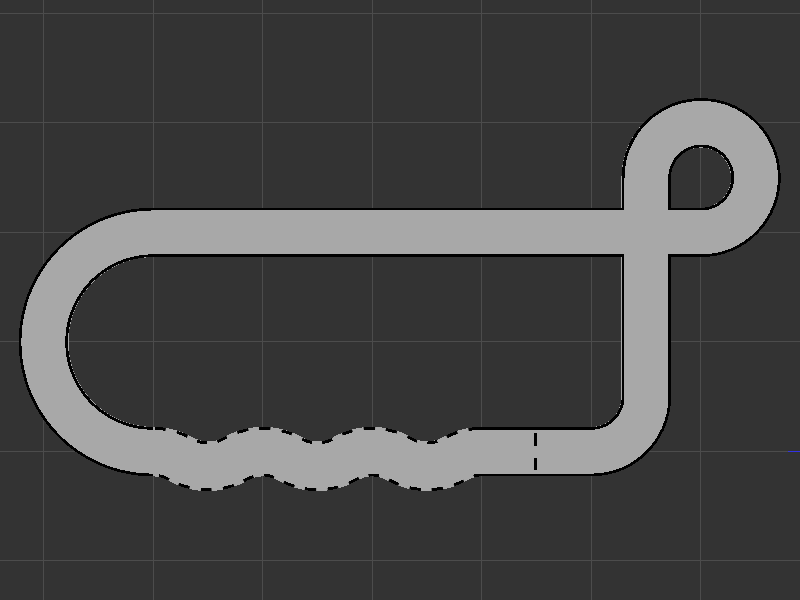
\includegraphics[width=0.80\textwidth]{demo3.png}
\caption{样例三}
\end{figure}
%<image src="demo3" name = "样例三"><middle>
\newpage
\section{样例函数}
为了使客户更快上手使用SCS,此处分别提供客户窗口样例绘制函数以及三个组别的样例决策函数。这些函数的源代码一并附在发布包中,具体参数可能略有不同。

客户窗口由freeglut创建,并在绘制前已设置好当前窗口句柄。本样例绘制函数使用OpenGL绘制简单的几何形体。

决策函数用简单的算法实现小车的巡线。但算法过于简单,对某些复杂路况还不能做出更智能的决策。

以下给出四个样例函数的代码,并解释其思路。
%在同本库一同发布的样例工程中,包含三个组别的样例决策函数。这几个决策函数用简单的算法实现小车的巡线。但算法过于简单,对某些复杂路况还不能做出更智能的决策。以下给出样例决策算法的代码,并解释其思路。

\subsection{样例绘制函数}

\begin{lstlisting}[language=C++]
void Display ()
{
	glTranslated (-0.5,-0.5,0.0);           // 平移
	glScaled (0.2,0.2,0.2);			// 缩放
	glColor3d (1.0,0.0,0.0);		// 颜色
	
	glBegin (GL_LINE_STRIP);		// 画线段
	for (int i=0; i<5; i++) {
		glVertex2d ((double)i,1.0);	// 线段坐标
		glVertex2d ((double)i,0.0);
	}
	glEnd ();				// 结束

	glLoadIdentity ();			// 复位
	glTranslated (0.0,0.5,0.0);		// 平移
	glColor3d (0.0,1.0,0.0);		// 颜色
	glRectd(-0.1,-0.1,0.1,0.1);		// 画矩形
}
\end{lstlisting}

该绘制函数在屏幕上绘制一条红色的折线和一个绿色的矩形。在此函数被SCS调用前默认已经设置好了窗口句柄,清除了颜色缓冲区,置模型空间当前矩阵为单位阵,置颜色为白色。故上述操作都不需要重复实现。客户窗口开启了双缓冲,在此函数被调用后默认刷新绘图指令缓冲,并交换两缓冲区指针。切勿重复执行此操作。详见\hyperlink{h672}{6.7.2}。\\

\newpage
\subsection{摄像头样例决策函数}
%<代码有行号,从0开始编号,tab宽度为8>
\begin{lstlisting}[language=C++]
void AI_Camera ()
{
	int i=25,j;
	int left,right,middle,dir,voltage,Threshold = 100;
	double speed;

	sGetGraph (graph);			    // 读取图像

	for (j=GRAPH_WIDTH/2; j>0; j--)		    // 搜索左侧黑点
		if (graph[i][j]<Threshold) break;
	left = j;
	for (j=GRAPH_WIDTH/2; j<GRAPH_WIDTH-1; j++) // 搜索右侧黑点
		if (graph[i][j]<Threshold) break;
	right = j;
	middle = (left+right)/2;

	dir = (middle-GRAPH_WIDTH/2) *3;	    // 计算舵机方向
	sSetServoDir (dir);
	
	speed = sGetSpeed();			    // 计算电机电压
	voltage = (int)((1.0-speed)*10.0 + 5.0);
	sSetMotor (voltage);
}
\end{lstlisting}

前几行申请变量,第6行调用接口获取图像。在此之前graph已实现分配好空间。

第8$\sim$14行为图像处理阶段。其算法是,从中点往两边扫描到第一个黑点时停止,并记录此点的坐标。据此计算其平均值得到赛道中心线的坐标middle。

第16$\sim$17行处理前轮角度信息。由于middle取值范围为0$\sim$GRAPH\_WIDTH,而舵机角度以0为中心,故将middle偏移GRAPH\_WIDTH/2得到舵机角度dir。比例系数3相当于PID控制中的P系数。

最后三行进行速度控制。先读取当前速度,取目标速度为1.0m/s,两者做差,再乘以比例系数。由于是位置式P控制,最后还有加上偏移量5.0。将上述计算结果调用接口函数传出。 \\

\newpage
\subsection{电磁样例决策函数}
\begin{lstlisting}[language=C++]
void AI_Electromagnetic ()
{
	int dir,voltage;
	double speed;
	double left,right;

	sVector pos(-0.1,0.3,0.05);
	left = sGetMagnetic (pos).GetX();    // 读取左侧磁感应强度

	pos.set(0.1,0.3,0.05);
	right = sGetMagnetic (pos).GetX();   // 读取右侧磁感应强度

	dir = (int)(fabs(right) - fabs(left))*5;    // 计算舵机方向
	sSetServoDir (dir);

	speed = sGetSpeed();			    // 计算电机电压
	voltage = (int)((1.0-speed)*10.0 + 5.0);
	sSetMotor (voltage);
}
\end{lstlisting}

第6$\sim$10行为调用接口函数读取磁感应强度的值,分别取左右各10厘米处,小车几何中心前30厘米处测量。在此只关心水平向右方向的磁感应强度分量。

第12$\sim$13行将左右二值做差,乘上比例系数,即得方向。

最后三行和摄像头的代码完全相同。 \\

\newpage
\subsection{光电样例决策函数}
\begin{lstlisting}[language=C++]
void AI_Balance ()
{
	static double Angle = 0.0;
	static double s = 0.0;
	int i,left,right,middle,dir,Threshold = 100;
	double voltage,speed;
	sVector AngularSpeed = sGetAngularSpeed ();
	Angle += AngularSpeed.GetX();

	speed = sGetSpeed();
	s += speed - 0.3;
	voltage = Angle*10.0 + AngularSpeed.GetX()*10.0 +
                  s*-20.0 + speed*-10.0;

	sGetLine (line);
	for (i=GRAPH_WIDTH/2; i>0; i--)		    // 搜索左侧黑点
		if (line[i]<Threshold) break;
	left = i;
	for (i=GRAPH_WIDTH/2; i<GRAPH_WIDTH-1; i++) // 搜索右侧黑点
		if (line[i]<Threshold) break;
	right = i;
	middle = (left+right)/2;		    // 计算方向
	
	dir = (middle-GRAPH_WIDTH/2) / 10;

	sSetMotorL (+dir-(int)voltage);
	sSetMotorR (-dir-(int)voltage);
}
\end{lstlisting}

第6$\sim$7行读取角速度的X分量(即前后摆动时产生的角速度),并积分出角度。

第9行读取速度,第10行积分出路程,并给路程一个固定的持续的偏差,迫使平衡控制算法误认为小车路程偏小,于是小车逐渐向前走。

第11行是平衡控制算法,该式以角度、角速度为内环PD控制,路程、速度为外环PD,篇幅所限恕不赘述。

第14$\sim$23行为图形识别部分与方向决策部分,算法与摄像头相同。

最后两行将平衡控制与方向控制相加输出给电机。

\newpage
\section{特别鸣谢}
\begin{figure}[!h]
\centering
\setcounter{subfigure}{0}
\subfigure[Bernhard Wymann]{
\includegraphics[width=0.3\textwidth]{berniw.jpg}} \\
\subfigure[M. R\'emi Coulom]{
\includegraphics[width=0.3\textwidth]{Remi-Coulom.jpg}} \\
\end{figure}
%<image src="berniw.jpg">
%<image src="Remi-Coulom.jpg">
\newpage
\section{鸣谢}
\begin{figure}[!h]
\centering
\setcounter{subfigure}{0}
\subfigure[月之子`丰子]{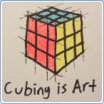
\includegraphics[width=0.3\textwidth]{fengzi.png}}
\subfigure[tju\_speed]{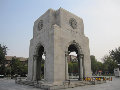
\includegraphics[width=0.3\textwidth]{tju_speed.jpg}} \\
\subfigure[☆\_。寒泉..+]{
\includegraphics[width=0.3\textwidth]{hanquan.jpg}}
\subfigure[恋May]{
\includegraphics[width=0.3\textwidth]{may.jpg}} \\
\subfigure[Andy Scout]{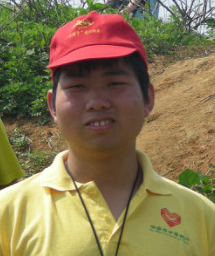
\includegraphics[width=0.3\textwidth]{andy.png}}
\subfigure[心之翼·自由]{
\includegraphics[width=0.3\textwidth]{free.jpg}} \\
\end{figure}

\section{附表}
\begin{center}
\begin{tabular}{ll}
\hline
项目	& 参数 \\
\hline
主窗口宽度	 & 800 \\
主窗口高度	 & 600 \\
滑动摩擦因数	 & 1.7 \\
重力加速度	 & $9.8\mathrm{m/s^2}$ \\
\hline
仿真步长	 & 1ms \\
FPS	 & 50 \\
AI调用虚拟频率	 & 50Hz \\
\hline
摄像头图像宽度	 & 320 \\
摄像头图像高度	 & 240 \\
摄像头视场长宽比    & 4:3 \\
\hline
线性CCD图像宽度	 & 128 \\
线性CCD图像高度	 & 1 \\
\hline
赛道厚度	 & 1cm \\
赛道宽度	 & 45cm(含边界线) \\
边界线宽度	 & 2.5cm \\
障碍高度	 & 0.5cm \\
坡道倾角	 & 15° \\
平衡组坡道倾角 & 12° \\
坡道过度长度	 & 10cm \\
虚线长度	 & 10cm \\
虚线空白长度	 & 10cm(起止处可能有误差) \\
最大赛道长度	 & 1000段 \\
\hline
底盘长度	 & 26cm \\
底盘宽度	 & 11cm \\
底盘高度	 & 0.5cm \\
左右轮距	 & 13.5cm \\
前后轮距	 & 20cm \\
A、D车底盘质量   & 0.5Kg  \\
平衡车底盘质量 & 0.25Kg \\
\hline
轮子质量   & 0.03Kg \\
A、D车轮子半径	 & 2.5cm \\
A、D车轮子宽度	 & 2.5cm \\
B车轮子半径	 & 3cm \\
B车转向轮宽度	 & 2.5cm \\
B车动力轮宽度	 & 4cm \\
\hline
电池长度	 & 13cm \\
电池宽度	 & 4cm \\
电池高度	 & 2cm \\
电池质量	 & 0.3Kg \\
\hline
\end{tabular}
\end{center}
\end{document}
